\chapter{Angles, Joints and Hands}
\label{C:angles-joints-hands}

Before I discuss my experiments training a model on hand motion data in the next chapter, I will first introduce some background related to modeling human hands, so we can understand many of the implementation choices I made.

\section{Parameterizing Hand Configurations}

To a first approximation, the human hand has 23 degrees of freedom.

\begin{figure}
    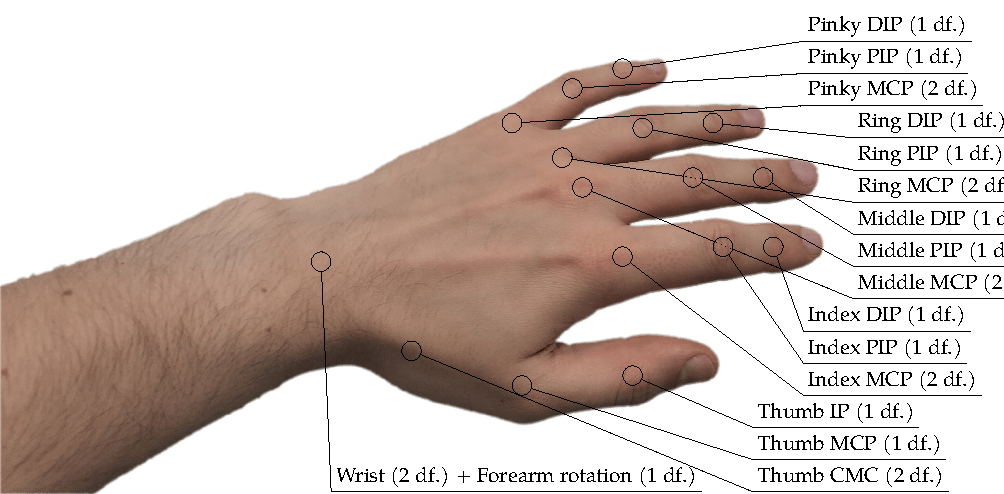
\includegraphics[width=\linewidth]{figures/hand-joints.pdf}
    \captionsetup{parskip=7pt}
    \caption[Joints of the hand]{Each hand has 16 joints - three per digit, plus the wrist.

    The wrist and the first joint on each digit (the metacarpophalangeal (MCP) joints) can rotate on two axes, and so each have 2 degrees of freedom. The rest (the proximal- and distal-interphalangeal (PIP \& DIP) joints) can only rotate on one axis, and have 1.

    This naive counting gives 22 degrees of freedom. In addition, we usually consider rotation of the forearm (about the longitudinal axis) to be part of the hand, modeling it as a third degree of freedom of the wrist, which brings the total to 23 degrees of freedom.}
    \label{fig:hand-joints}
\end{figure}

As we can see in \Cref*{fig:hand-joints},

Considering that different combinations of joint angles can have very {\Symbola\Large\Large\symbol{"1F91E}} different {\Symbola\Large\Large\symbol{"1F919}} meanings {\Symbola\Large\Large\symbol{"1F44C}}, animators have a lot of work to do when bringing a digital character to life. Small mistakes can cause a character to look unnatural, but in many scenes getting the hands perfect goes unnoticed.

It is not so straightforward to assign an angle to each of those 23 degrees of freedom. There are a variety of different parameterizations of the joints we might choose from, and additionally we have the option of placing constraints on the range of values that the angles can take. In this section we will discuss some of the most common parameterizations, and the pros and cons of each.

\subsection{Euler Angles}

Euler angles are the most common parameterization for human joints. They are also the simplest to understand. Each joint is assigned three angles, one for each axis of rotation. The axes are usually chosen to be the x, y, and z axes of the coordinate system, but they can be chosen to be any three axes that are orthogonal to each other.  For example, the axes could be chosen to be the axes of the joint itself, or the axes relative to the parent joint. The order in which the rotations are applied is also important. The most common order is to apply the rotations in the order $z$, $y$, $x$, but they can be applied in any order.

This parameterization has the topology $S^1 \times S^1 \times S^1 ≅ T^3$, where $S^1$ is the circle of angles. However, the space of rotations $SO(3)$ itself has topology $S^3$, so the Euler angle parameterization cannot be perfect. In particular, there must be singularities.

The principle advantage of the Euler angle parameterization is that it is easy to understand and implement. The principle disadvantages are due to the singularities:
\begin{enumerate}
    \item there may be multiple sets of Euler angles that correspond to the same rotation
    \item as a result, we cannot easily interpolate between two configurations that are close together but have different Euler angles
\end{enumerate}

For example, if we rotate a joint by $90^\circ$ about the $x$ axis, and then by $90^\circ$ about the $y$ axis, we will get the same rotation as if we had rotated by $90^\circ$ about the $y$ axis, and then by $90^\circ$ about the $x$ axis. \TODO{ Euler angle figure }

If we tried to interpolate between these two configurations, we would get a rotation that is not the same as either of the two configurations. This occurs because the Euler angle parameterization is not a smooth function.

\subsection{Axis-Angle}

An alternative parameterization is to use an axis-angle representation. In this representation, each joint is assigned a unit vector and an angle. The unit vector specifies the axis of rotation, and the angle specifies the amount of rotation. The axis-angle representation has the topology $S^2 \times S^1$, where $S^2$ is the sphere of unit vectors. Because topology still does not match the space of rotations $SO(3)$, there are still singularities. However




\section{Loss Functions for learning angles}

In \Cref{C:background} I introduced some loss functions such as the Mean Squared Error (MSE), which predicts the posterior expectation $\mathbb{E}(y | x)$. In this section I will discuss some other loss functions, that are commonly used for learning data which sits on .

A variant of this is the \textit{angular} mean-squared-error, which I will use later on in \Cref{C:hand-model}.
\newcommand{\amse}{L_{\theta\text{-MSE}}}
\begin{align}
\label{notation:amse}
\begin{split}
    \fdef{\amse}{\R^{N×D}×\R^{N×D}}{\R} \\
    \amse&(y, \hat{y})_{ni} ≝ \frac{1}{N} \sum_n\left[ \sum_i (\sin y_{ni} - \sin \hat{y}_{ni})^2 + (\cos y_{ni} - \cos \hat{y}_{ni})^2 \right]
\end{split}
\end{align}
Here $y$ and $\hat{y}$ are vectors of angles, and the error is defined in terms of the squared arc length between their corresponding components. This loss function is equivalent to maximising the likelihood of a von Mises distribution, the derivation for which can be found in \Cref{C:angles-joints-hands}. This is useful when we want to model angles, for example when we want to predict the orientation of a hand, which we will do in \Cref{C:hand-model}.

\TODO{ Derivation of $\theta$-MSE minimizing von-mises distribution }
